%!TEX program = xelatex
% 完整编译: xelatex -> biber/bibtex -> xelatex -> xelatex
\documentclass[11pt,a4paper]{article}

\title{Numerical Analysis HW5
}
\author{Jinchen Wang}
\date{2022/12/12}
% 本文档命令
\usepackage{amssymb}
\usepackage{mathrsfs}
\usepackage{geometry}
\usepackage{graphicx}
\usepackage{array}
\usepackage{cite}
\usepackage{float}
\usepackage{subcaption}
\usepackage{longtable}
\newcommand{\ccr}[1]{\makecell{{\color{#1}\rule{1cm}{1cm}}}}
\usepackage{algorithm}
\usepackage{algorithmic}
\usepackage{listings}
\usepackage{url}
\usepackage{tikz}
\usetikzlibrary{positioning, shapes.geometric}
%\usepackage{pgfplots}
\usepackage{amsmath,amsfonts,bm}
%\usepackage{ctex}
\usepackage[amsmath,thmmarks,framed]{ntheorem}
\theoremstyle{plain}
\theorembodyfont{\small}
\usepackage{framed}
\usepackage{minted}
\usepackage{color}
\usepackage{booktabs}
\definecolor{gray}{rgb}{0.6,0.6,0.6}
\renewcommand*\FrameCommand{{\color{gray}\vrule width 5pt \hspace{10pt}}}
\newframedtheorem{defn}{Definition}
\newframedtheorem{thm}{Theorem}
\newframedtheorem{lem}{Lemma}
\newframedtheorem{prop}{Property}
\newframedtheorem{clou}{Conclusion}
\newcommand\R {\mathbb{R}}
\newcommand\T {\mathbb{T}}
\newcommand\mx {\bm x}
\newcommand\my {\bm y}
\newcommand\mg {\bm g}
\geometry{a4paper,scale=0.77}
\lstset{
		columns=fullflexible, 
		numbers=left,
		numberstyle=\tiny\color{gray}, 
		commentstyle=\color[cmyk]{1,0,1,0}, 
		escapeinside=``, 
		breaklines, 
		extendedchars=false, 
		xleftmargin=1em,xrightmargin=1em, aboveskip=1em, 
		tabsize=4, 
		showspaces=false
		keywordstyle=\color[RGB]{40,40,255}, 
		numberstyle=\footnotesize\color{darkgray},         
		commentstyle=\it\color[RGB]{0,96,96}, 
		stringstyle=\rmfamily\slshape\color[RGB]{128,0,0}, 
		showstringspaces=false, 
		language=python, 
		backgroundcolor=\color[RGB]{245,245,244}, 
		frame=shadowbox,
	}

\makeatletter
\@addtoreset{equation}{section}
\makeatother
\renewcommand{\theequation}{\arabic{section}.\arabic{equation}}
\usepackage{tabularx}
\usepackage{indentfirst}
\usepackage{fontspec}
\setmainfont{Times New Roman}


\begin{document}

\maketitle

\section*{Theoretical Questions}
\section*{Question 1}
\noindent Proof:\\
(1) Positive Definite.
\begin{equation}
    \begin{aligned}
        \forall u \in C[a,b],\;	\left \langle {u,v}\right \rangle = \int_{a}^{b} p(x)u(x)\overline{u(x)} dx =  \int_{a}^{b} p(x)u(x)^2 dx > 0
    \end{aligned}
\end{equation}

\noindent(2) Regularity.
\begin{equation}
    \begin{aligned}
        \left \langle {u,u}\right \rangle = 0 \Leftrightarrow p(x)u(x)^2 = 0 \Leftrightarrow u = 0
    \end{aligned}
\end{equation}

\noindent(3) Additivity.
\begin{equation}
    \begin{aligned}
        \left \langle {u+w,v}\right \rangle &= \int_{a}^{b} p(x)(u(x)+w(x))\overline{v(x)} dx\\
        &= \int_{a}^{b} p(x)u(x)\overline{v(x)}dx+ \int_{a}^{b} p(x)w(x)\overline{v(x)}dx\\
        &=  \left \langle {u,v}\right \rangle + \left \langle {w,v}\right \rangle
    \end{aligned}
\end{equation}

\noindent(4) Conjugate Symmetry.
\begin{equation}
    \begin{aligned}
        \left \langle {u,v} \right \rangle &= \int_{a}^{b} p(x)u(x)\overline{u(x)} dx\\
        &= \overline{\int_{a}^{b} \overline{p(x)u(x)\overline{v(x)}}dx}\\
        &= \overline{\int_{a}^{b} p(x)\overline{u(x)}v(x)}\\
        &= \overline{ \left \langle {v,u} \right \rangle}
    \end{aligned}
\end{equation}

\noindent(5) Norm Positive Definite.
\begin{equation}
\|u\|_2=\left[\int_a^b \rho(x)|u(x)|^2 \mathrm{~d} x\right]^{1 / 2} \geq 0
\end{equation}
\noindent

\noindent(6) Norm Regularity.
\begin{equation}
\|u\|_2=0 \Leftrightarrow \rho(x)|u(x)|^2=0 \Leftrightarrow|u(x)|^2=0 \Leftrightarrow u=0
\end{equation}

\noindent(7) Norm Inequality.
\begin{equation}
\begin{aligned}
\forall u, v \in \mathcal{C}[a, b], \quad\|u+v\|_2 & =\left[\int_a^b \rho(x)|u(x)+v(x)|^2 \mathrm{~d} x\right]^{1 / 2} \\
& \leq\left[\int_a^b \rho(x)|u(x)|^2 \mathrm{~d} x\right]^{1 / 2}+\left[\int_a^b \rho(x)|v(x)|^2 \mathrm{~d} x\right]^{1 / 2} \\
& =\|u\|_2+\|v\|_2
\end{aligned}
\end{equation}

\section*{Question 2}
\subsection*{(1)}
\noindent We let $p(x) = \frac{1}{\sqrt{1-x^2}}$ and the First Chebyshev Polynomial is,
\begin{equation}
T_n(x)=\cos (n \arccos x), \quad x \in[-1,1], \quad n=0,1,2, \ldots
\end{equation}
\noindent therefore,
\begin{equation}
\begin{aligned}
\forall m, n \quad\left\langle T_m, T_n\right\rangle & =\int_{-1}^1 \frac{1}{\sqrt{1-x^2}} T_m(x) \overline{T_n(x)} \mathrm{d} x \\
& =\int_{-1}^1 \frac{1}{\sqrt{1-x^2}} \cos (m \arccos x) \cos (n \arccos x) \mathrm{d} x \\
\text{Let }\theta=\arccos x,\\
& =\int_0^\pi \cos (m \theta) \cos (n \theta) \mathrm{d} \theta \\
& =\frac{1}{2} \int_0^\pi[\cos (m+n) \theta+\cos (m-n) \theta] \mathrm{d} \theta \\
\end{aligned}
\end{equation}
Thus,
\begin{equation}
    \begin{aligned}
        \quad\left\langle T_m, T_n\right\rangle = \begin{cases}0, & m \neq n \\
\pi, & m=n=0 \\
\frac{\pi}{2}, & m=n \geq 1\end{cases}
    \end{aligned}
\end{equation}
Hence, the chebyshev polynomials are orthogonal.

\subsection*{(2)}
\begin{equation}
T_0^*(x)=\sqrt{\frac{1}{\pi}}, \quad T_1^*(x)=\sqrt{\frac{2}{\pi}} x, \quad T_2^*(x)=\sqrt{\frac{2}{\pi}}\left(2 x^2-1\right) .
\end{equation}

\section*{Question 3}
\subsection*{(1) Orthonormal Polynomials}
\noindent According to the previous question, we have orthonormal polynomials,\\
\begin{equation}
T_0^*(x)=\sqrt{\frac{1}{\pi}}, \quad T_1^*(x)=\sqrt{\frac{2}{\pi}} x, \quad T_2^*(x)=\sqrt{\frac{2}{\pi}}\left(2 x^2-1\right) .
\end{equation}
Therefore, the approximation of the circular arc is given as follows,\\
\begin{equation}
\begin{aligned}
\varphi(x) & =\left\langle y, T_0^*\right\rangle T_0^*+\left\langle y, T_1^*\right\rangle T_1^*+\left\langle y, T_2^*\right\rangle T_2^* \\
& =\frac{2}{\pi}+0-\frac{4}{3 \pi}\left(2 x^2-1\right) \\
& =-\frac{8}{3 \pi} x^2+\frac{10}{3 \pi} 
\end{aligned}
\end{equation}

\subsection*{(2) Normal Equation}
\noindent Let $\phi(x) = a_0 + a_1x+a_2x^2$,\\
\begin{equation}
\left[\begin{array}{ccc}
\langle 1,1\rangle & \langle 1, x\rangle & \left\langle 1, x^2\right\rangle \\
\langle x, 1\rangle & \langle x, x\rangle & \left\langle x, x^2\right\rangle \\
\left\langle x^2, 1\right\rangle & \left\langle x^2, x\right\rangle & \left\langle x^2, x^2\right\rangle
\end{array}\right]^T\left[\begin{array}{l}
a_0 \\
a_1 \\
a_2
\end{array}\right]=\left[\begin{array}{c}
\langle y, 1\rangle \\
\langle y, x\rangle \\
\left\langle y, x^2\right\rangle
\end{array}\right]
\end{equation}
that is,\\
\begin{equation}
\left[\begin{array}{ccc}
\pi & 0 & \frac{\pi}{2} \\
0 & \frac{\pi}{2} & 0 \\
\frac{\pi}{2} & 0 & \frac{3 \pi}{8}
\end{array}\right]^T\left[\begin{array}{l}
a_0 \\
a_1 \\
a_2
\end{array}\right]=\left[\begin{array}{c}
2 \\
0 \\
\frac{2}{3}
\end{array}\right]
\end{equation}
\noindent Solving these linear equations, we have,
\begin{equation}
    a_0 = \frac{10}{3\pi},\; a_1 = 0,\;a_2 = \frac{-8}{3\pi}
\end{equation}

\noindent Therefore,\\
\begin{equation}
    \phi(x) = -\frac{8}{3 \pi} x^2+\frac{10}{3 \pi}
\end{equation}

\section*{Question 4}
\subsection*{(1)}
\noindent Let the input $u_1 = 1, u_2 = x, u_3 =x^2$, by Gram-Schmidt,
\begin{equation}
    \begin{aligned}
    & v_1=u_1\\
    & u_1^*=v_1 /\left\|v_1\right\|_2=v_1 / \sqrt{12}=\frac{1}{2 \sqrt{3}} \\
    & v_2=u_2-\left\langle u_2,u_1^*\right\rangle u_1^*=x-\frac{13}{2}\\
    & u_2^*=v_2 /\left\|v_2\right\|_2=\frac{1}{\sqrt{143}}\left(x-\frac{13}{2}\right) \\
    & v_3=u_3-\left\langle u_3, u_1^*\right\rangle u_1^*-\left\langle u_3, u_2^*\right\rangle u_2^*=x^2-\frac{325}{6}-13 \times\left(x-\frac{13}{2}\right)=x^2-13 x+\frac{91}{3} \\
    & u_3^*=v_3 /\left\|v_3\right\|_2=\frac{\sqrt{3}}{\sqrt{4004}}\left(x^2-13 x+\frac{91}{3}\right)
    \end{aligned}
\end{equation}

\subsection*{(2)}
\noindent By corollary 5.25, the best approximation $\hat{\varphi(x)}$ is the projection on the orthonormal basis.\\
\begin{equation}
    \begin{aligned}
    \hat{\varphi}(x) & =\left\langle y, u_1^*\right\rangle u_1^*+\left\langle y, u_2^*\right\rangle u_2^*+\left\langle y, u_3^*\right\rangle u_3^* \\
    & =\frac{831}{\sqrt{3}} u_1^*+\frac{589}{\sqrt{143}} u_2^*+\frac{12068 \sqrt{3}}{\sqrt{4004}} u_3^* \\
    & \approx 9.042 x^2-113.4266 x+386.0013
    \end{aligned}
\end{equation}

\subsection*{(3)}
\noindent \textbf{Orthonormal Polynomials   :}\\
\indent For different $y_i$s, the orthonormal basis $\{u_1^*,u_2^*,u_3^*\}$ can be reused, while the computation of the projection can not. So we only need to recompute $ \hat{\varphi}(x) & =\left\langle y, u_1^*\right\rangle u_1^*+\left\langle y, u_2^*\right\rangle u_2^*+\left\langle y, u_3^*\right\rangle u_3^*$.\\
\noindent \textbf{Normal Equation:}\\
\indent For different $y_i$s, the coefficient matrix can be reused, but we have to recompute the vectors righthand, which requires us to compute n inner matrices and to solve the linear equations.\\
\noindent \textbf{The advantage of orthonormal polynomials over normal equations:}\\
\noindent(1) The orthonormal basis can be reused in different approximation.\\
\noindent(2) When using \textbf{ORTHONORMAL POLYNOMIALS}, we only need to recompute n inner products, while using \textbf{NORMAL EQUATION} requires us to additionally solve linear equation, which increases the amount of calculation and the condition number.
\indent 

\section*{Programming Problems}
\noindent\textbf{MATLAB is utilized for this part.}
\section*{Program 1}
\noindent The input is x, y and we can find the coefficient in the output a.
\begin{equation}
    a = [2.1757 , 2.6704, -0.2384]^T
\end{equation}
Thus, the best approximation is,
\begin{equation}
    \hat{\varphi(x)} = 2.1752 + 2.6704x - 0.2384x^2
\end{equation}
\begin{figure}[H]
    \centering
    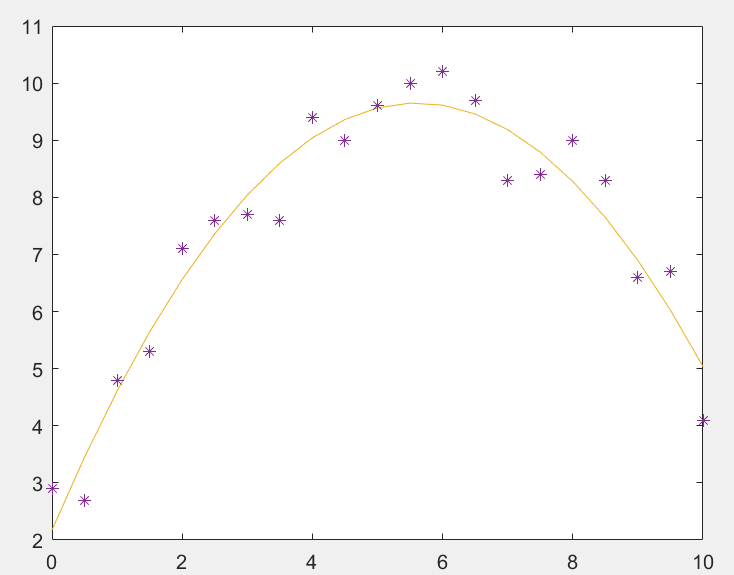
\includegraphics[width=10cm]{1.png}
    \caption{The approximation by Normal Equation}
    \label{fig:1L}
\end{figure}

\section*{Program 2}
After QR Factorization for the Vandermonde Matrix and solving $R_1*x = c$, we also have,
\begin{equation}
    a = [2.1757 , 2.6704, -0.2384]^T
\end{equation}
Thus, the best approximation is,
\begin{equation}
    \hat{\varphi(x)} = 2.1752 + 2.6704x - 0.2384x^2
\end{equation}
\indent which is the same as in Program 1, verifying the correctness.\\
\begin{figure}[H]
    \centering
    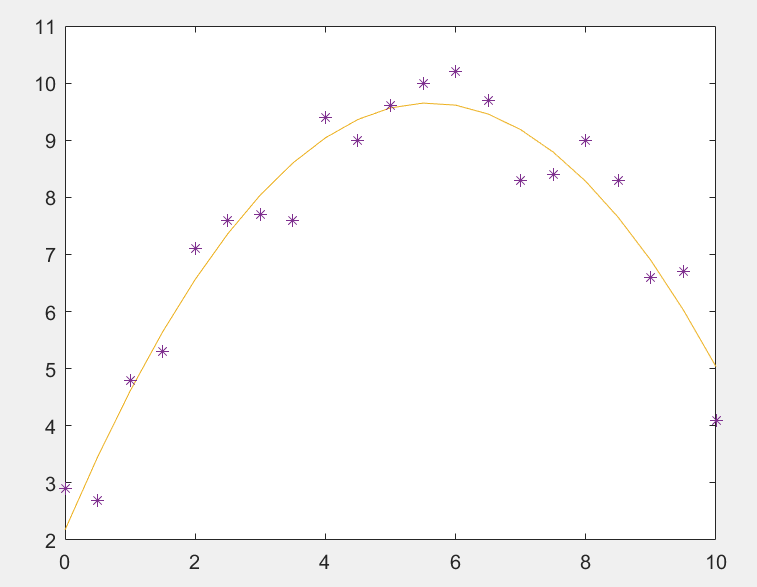
\includegraphics[width=10cm]{2.png}
    \caption{The approximation by QR}
    \label{fig:1L}
\end{figure}
\noindent Besides,\\
the condition number of G is 4.585153881696407e+04,\\
the condition number of R1 is 2.141297242723767e+02.\\
\indent Apparently, the condition number of the Gram matrix is larger than the condition number of the matrix $R_1$ corresponding to the QR Factorization.
\end{document}
